\documentclass{article}
\usepackage[T1]{fontenc}
\usepackage{lmodern}
\usepackage{graphicx}
\usepackage{amsmath,amssymb}
\usepackage[a4paper,margin=2cm]{geometry}
\usepackage[absolute,overlay]{textpos}
\setlength{\TPHorizModule}{1mm}
\setlength{\TPVertModule}{1mm}
\usepackage[indonesian]{babel}
\usepackage{hyperref}
\setlength{\emergencystretch}{2em}
% unit: Halaman 21

\begin{document}

% === Halaman 21 (llm) ===

\textbf{The IEEE Koji Kobayashi Computers and Communications Award}\
The 1999 award was given to Diffie, Hellman and Merkle \"For the revolutionary invention of public key cryptosystems which form the foundation for privacy, integrity and authentication in modern communication systems.\"
The 2000 award was given to Rivest, Shamir and Adleman \"For the revolutionary invention of the RSA public key cryptosystem which is the first to be widely-adopted.\"

\vspace{50mm}

From left to right: Adi Shamir, Ron Rivest, Len Adleman, Ralph Merkle, Martin Hellman, and Whit Diffie (Picture courtesy of Eli Biham, taken at the presentation on Monday August 21 at Crypto 2000, an IACR conference)

\centering{Rinaldi M/II4020 Kriptografi}\
\centering{\textcolor{red}{Sumber: http://www.merkle.com/merkleDir/KobayashiAward.html}}

% deskripsi: Foto para penerima Penghargaan IEEE Koji Kobayashi Computers and Communications, yang terdiri dari Adi Shamir, Ron Rivest, Len Adleman, Ralph Merkle, Martin Hellman, dan Whit Diffie.
% bbox normalisasi: [0.1800, 0.2600, 0.7440, 0.7760]
\begin{textblock*}{118.44mm}(37.80mm,77.22mm)
\noindent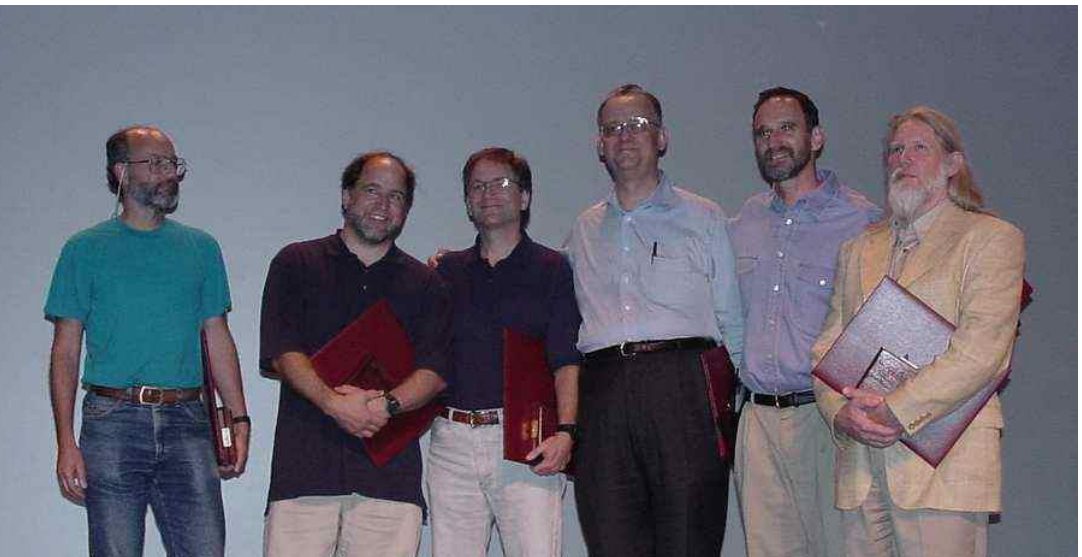
\includegraphics[width=118.44mm,height=153.25mm]{../../images/llm/page_021_img_01.png}%
\end{textblock*}

\end{document}
